\documentclass[12pt]{article}
\setlength{\textwidth}{17cm}
\setlength{\textheight}{24cm}
\setlength{\topmargin}{-2cm}
\setlength{\footskip}{1cm}
\setlength{\evensidemargin}{0cm}
\setlength{\oddsidemargin}{0cm}
\setlength{\parindent}{0cm}

\usepackage{allrunes}
\usepackage{amsmath}
\usepackage{amsthm}
\usepackage{amssymb}
\usepackage[english]{babel}
\usepackage[T1]{fontenc}
\usepackage[utf8]{inputenc}
%\usepackage{fixltx2e}
\usepackage{multirow}

\usepackage[hyphens]{url}
\usepackage[unicode,colorlinks=true,breaklinks]{hyperref}
%\usepackage[dvips]{hyperref}
%should display links, but it does not work with \H accent
%and formulas in section titles

\hypersetup{colorlinks,linkcolor=blue,urlcolor=magenta,citecolor=magenta}
%Breaks long url`s in text, while keeping it one link:

\usepackage{amsfonts}
\usepackage{amsthm}
\usepackage{amssymb}


\theoremstyle{plain}
\usepackage{graphicx}

%\usepackage{gensymb}
\usepackage{float}

% For bra-ket notation
\usepackage{braket}

%% New commands
\newcommand{\dd}{\textrm{d}}

%% Pauli matrices
\newcommand{\sigx}{\sigma_x}
\newcommand{\sigy}{\sigma_y}
\newcommand{\sigz}{\sigma_z}

\newcommand{\paulix}{
    \left( \begin{array}{cc}
        0 & 1 \\
        1 & 0
    \end{array}
    \right)
}

\newcommand{\pauliy}{
    \left( \begin{array}{cc}
        0 & -i \\
        i & 0
    \end{array}
    \right)
}

\newcommand{\pauliz}{
    \left( \begin{array}{cc}
        1 & 0 \\
        0 & -1
    \end{array}
    \right)
}


\begin{document}
\title{12th exam item}
\author{András Mátyás Biricz}

\maketitle


\newpage
\begin{abstract}
    Neurális hálók - teljesen összekötött neurális hálók, konvolúciós neurális hálók, backpropagation, optimizerek (SGD, Adam), batch normalisation, autoencoderek, word2vec
    
    Neural networks - multilayer perceptrons (fully-connected feedforward neural networks), convolutional neural networks, backpropagation, optimizers (SGD, Adam), batch normalization, autoencoders, word2vec
\end{abstract}

\section{Introduction}

In special tasks like speech recognition or object detection machine learning methods could not achieve the desired performance, could not generalize well and often failed to process high-dimensional data. This motivated a different approach that has led to the widespread use of neural networks. However, the basic concepts of deep learning have a long history dated back to the middle of the 20th century. To introduce the fundamentals of deep learning, I will follow this excellent book of \hyperlink{Deeplea_Goodfellow}{Goodfellow et al (2016)}.

\section{Fundamentals of neural networks}

\subsection{Traditional architecture}

\subsubsection{Multilayer perceptron}

The concept of the perceptron was founded by \hyperlink{Deeplea_Rosenblatt_1}{Rosenblatt F. (1958),} \hyperlink{Deeplea_Rosenblatt_2}{(1962)} and is a simple model for making decision based on learned parameters. In a modern sense, the perceptron is an algorithm for a learning binary classifier, more presicely a function that maps its input $\textbf{x}$ (real valued) to an output value $f(\textbf{x})$:

\begin{equation}
f(\mathbf{x}) = \begin{cases}1, & \text{if }\ \mathbf{w} \cdot \mathbf{x} + b > 0,\\0, & \text{otherwise,}\end{cases}
\end{equation}
where $\textbf{w}$ is a vector of real-valued weights, $\textbf{w} \cdot \textbf{x}$ is the dot product $\sum_{i=1}^m w_i x_i$, where $m$ is the number of inputs to the perceptron, and $b$ is the bias. The definition of the neuron that builds up the modern neural networks slightly differs, while the perceptron has a Heaviside-function for its activation, the neuron can have any non-linear function for it.

The feedforward neural networks (or multilayer perceptrons) are the classical deep learning models that can have many layers with different numbers of neurons in each. The information flows through the network from the input as the functions are being evaluated. The name network originates from that each layer is connected to the previous one or the input. The output is the composition of functions. In case of 3 layers $f^{(1)}$, $f^{(2)}$ and $f^{(3)}$ are the outputs of each layer, respectively, and the final output can be constructed by: $f(\textbf{x}) =  f^{(3)}\{f^{(2)}[f^{(1)}(\textbf{x})]\}$. The depth of the model is given by the length of this chain and the model can have the \textit{deep} attribute if it has many layers.

The importance of the non-linear activation lies in the fact that if the activations of the neurons are just linear maps, the whole network could be simplified into a linear map with transformations, which of course would not be able to learn non-linear behaviour. Additionally, the learning method called backpropagation could not be carried out in this case, since the derivative of the output function would be a constant and would not reflect any properties of the input or the representation of the input by the hidden layers. To extend the model it is inevitable to apply different types of non-linear functions as activation. The most general ones are the following:

\begin{itemize}
	\item sigmoid: 
	\begin{equation}
	f(x) = \frac{1}{1 + e^{-x}},
	\end{equation}		
	\item rectified linear unit (ReLU):
	\begin{equation}
	f(x) = x^+ = max(0,x),
	\end{equation}
	\item softmax:
	\begin{equation}
	f(\mathbf{x})_i = \frac{e^{x_i}}{\sum_{j=1}^M e^{x_j}}.
	\end{equation}
\end{itemize}

The softmax activation is a function that takes $M$ real numbers as input and normalizes them into a probabilistic distribution. This property makes it capable to use it in case of probabilistic multiclass prediction.

Usually, neural networks are used in supervised learning. During the training process the output of the network $f^*(\textbf{x})$ is to be matched with the known label $y=f(x)$, therefore the network provides function approximation. Only the last layer is involved directly, the behaviour of the rest is not tested, that is why those are called hidden layers.

\subsubsection{Backpropagation}

At the initialization of the neural network the weights are set for each neuron (randomly or by sampling from a distribution). When the inputs are loaded and passed through the whole network, it will predict with this initial setup. To modify the weights, so to make the network learn features, feedback should be sent back through every layer describing the goodness of the function approximation (prediction). This process is called backpropagation. In order to adjust the weights from the information of the backpropagated error a (stable) numerical optimization method should be used. This is usually the gradient descent that can be tracked on figure \ref{grad_desc_fig_1}, which consist of the following step repeated iteratively:

\begin{equation}
W = W - \alpha \frac{ \partial L}{ \partial W},
\end{equation}

\begin{equation}
b = b - \alpha \frac{ \partial L}{ \partial b},
\end{equation}
where $W$ denotes the weights, $b$ the biases, $\alpha$ is the learning rate and $L$ is the loss function. The partial derivatives of the loss function with respect to the weights and biases can be calculated using the chain rule for every layer of the network. The analytical form of the result depends on the chosen loss function and will have dependent variables of the inputs and activations in each layer. 

The general, more detailed calculation process can be read below and tracked on figure \ref{backprop_fig}:

\begin{equation}
\frac{\partial E}{\partial w_{ij}} = \frac{\partial E}{\partial o_{j}} \frac{\partial o_{j}}{\partial w_{ij}}
= \frac{\partial E}{\partial o_j} \frac{\partial o_j}{\partial\text{net}_j} \frac{\partial \text{net}_j}{\partial w_{ij}},
\end{equation}


\begin{equation}
\frac{\partial \text{net}_j}{\partial w_{ij}} = \frac{\partial}{\partial w_{ij}} \left(\sum_{k=1}^n w_{kj} o_k\right) = \frac{\partial}{\partial w_{ij}}  w_{ij} o_i= o_i,
\end{equation}

\begin{equation}
\frac{\partial o_j}{\partial\text{net}_j} = \frac {\partial  \varphi(\text{net}_j)}{\partial \text{net}_j},
\end{equation}
where different notations are used: $E=L$ denotes the loss function (error), $w_{ij}$ the weights for $i$th neuron found in the $j$th layer, net$_j$ is the transfer function, so the activations from the previous layer or the input for the first layer, and $o_i$ is the activation calculated from the transfer function with a pointwise nonlinearity $\varphi$. 

Further details of the derivation can be found on this page\footnote{\url{https://en.wikipedia.org/wiki/Backpropagation}.}.

\begin{figure}[h!]
    \centering
	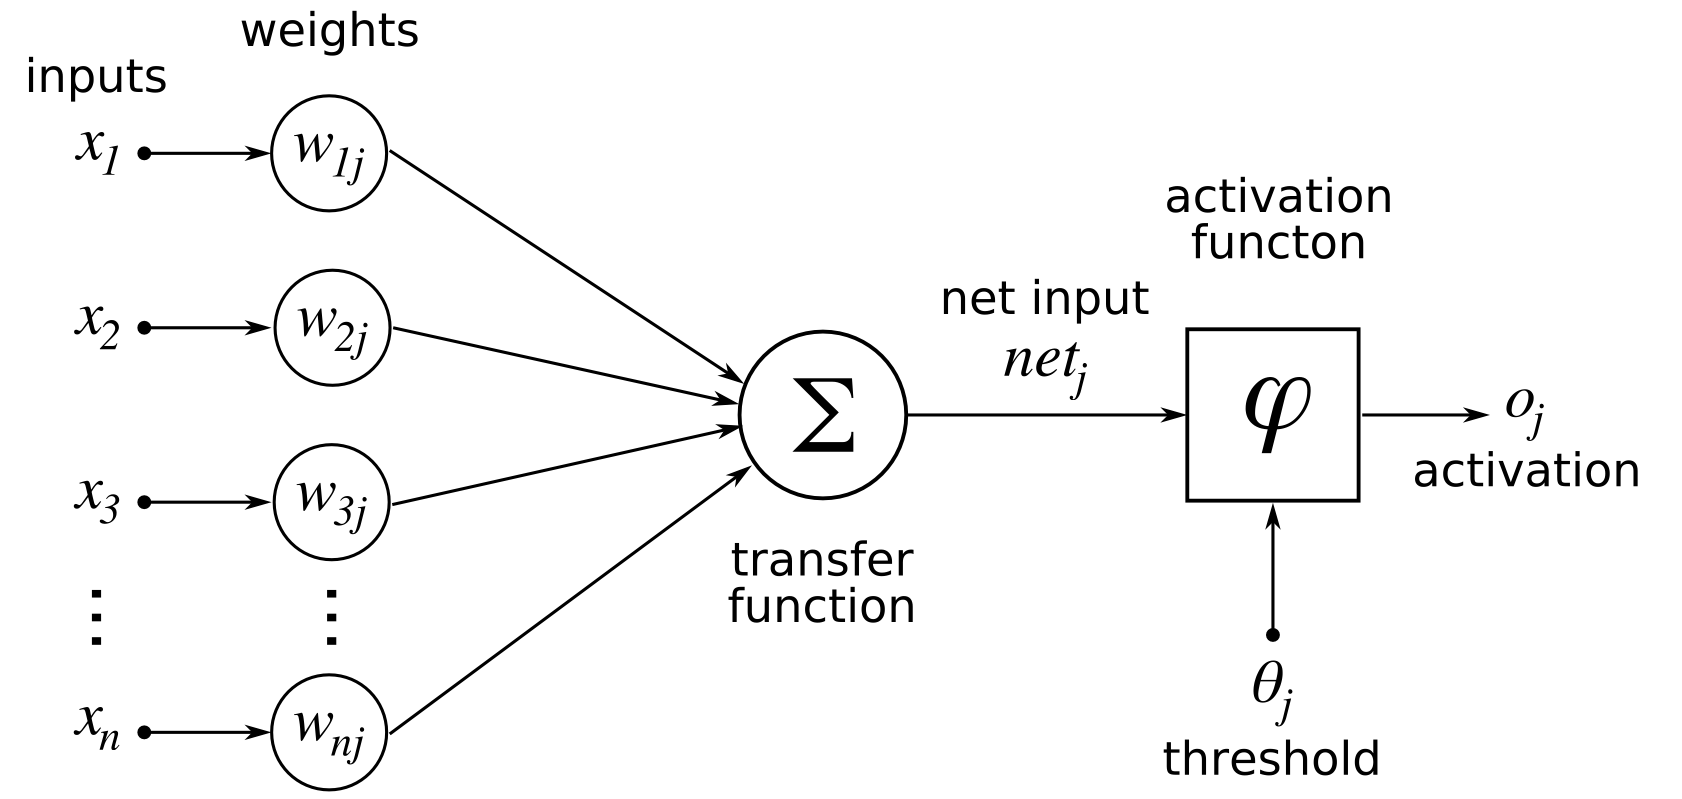
\includegraphics[width=.9\linewidth]{media/ArtificialNeuronModel_english.png}
	\caption{Diagram of the neural network with the notations used for the derivation of the backpropagation. The source was accessed in May 2019 (\url{https://en.wikipedia.org/wiki/Backpropagation\#/media/File:ArtificialNeuronModel_english.png}).}
	\label{backprop_fig}
\end{figure}

\subsubsection{Optimizers}

So the training of the neural networks can be done with gradient descent (see figure \ref{grad_desc_fig_1}), but due to the non-linear behaviour of the networks the loss functions will be non-convex (as seen on figure \ref{grad_desc_fig_2}), which is a huge difference compared with the case of optimizing the machine learning methods. Consequently, the training process will be done using iterative, gradient-based optimizers that merely drive the loss functions to very low values. Generally, the whole train set is shuffled, then divided into small parts, called mini-batches of size usually from 16 to 256. This has the advantage of adding extra noise to the optimization process and probably helps to avoid falling into local minima. 

\begin{figure}[h!]
    \centering
	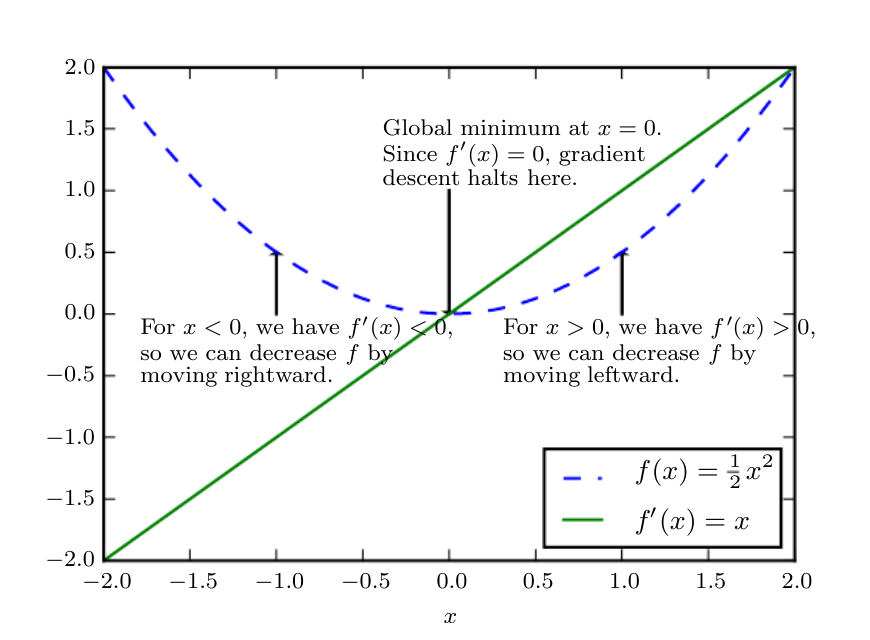
\includegraphics[width=.7\linewidth]{media/grad_desc_fig1.png}
	\caption{Visualization of the gradient descent algorithm how it takes advantage of the derivatives of a function in order to find the minimum value. The figure is taken from \protect\hyperlink{Deeplea_Goodfellow}{Goodfellow et al (2016)}.}
	\label{grad_desc_fig_1}
\end{figure}

To be more precise, there are three different types of the gradient-descent algorithm.

\begin{itemize}
	\item \textbf{Stochastic gradient descent:} calculates the error and updates the model for each example in the input data.
	\item \textbf{Batch gradient descent:} calculates the error for each example in the training set, but only updates the model after all examples have been evaluated.
	\item \textbf{Mini-batch gradient descent:} mixture of the previous two, splits the training set into small batches in which the error of the model is calculated then updated.
\end{itemize}

\begin{figure}[h!]
    \centering
	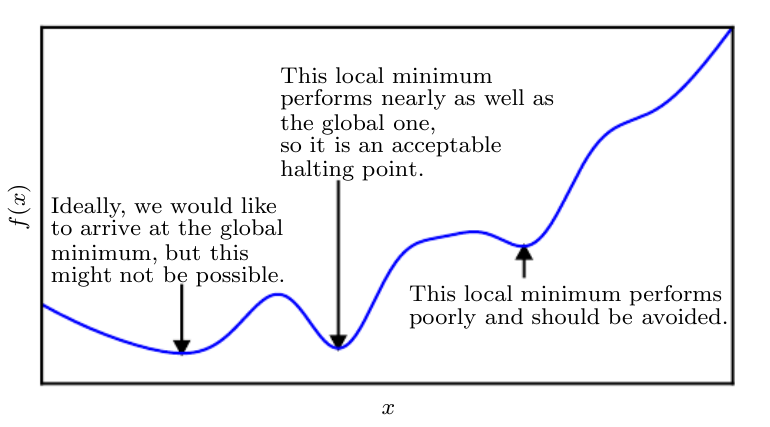
\includegraphics[width=.7\linewidth]{media/grad_desc_fig2.png}
	\caption{A typical case of a non-convex loss function during the training of a neural network. The figure is taken from \protect\hyperlink{Deeplea_Goodfellow}{Goodfellow et al (2016)}.}
	\label{grad_desc_fig_2}
\end{figure}

A very efficient and commonly used extension to the stochastic gradient descent (SGD) is the Adam optimizer. It takes advantage of the following two other extensions of the SGD:

\begin{itemize}
	\item \textbf{Adaptive Gradient Algorithm (AdaGrad):} maintains a per-parameter learning rate that improves performance on problems with sparse gradients (e.g. natural language and computer vision problems).
	\item \textbf{Root Mean Square Propagation (RMSProp):} also maintains per-parameter learning rates that are adapted based on the average of recent magnitudes of the gradients for the weight (e.g. how quickly it is changing). This means the algorithm does well on online and non-stationary problems (e.g. noisy).

\end{itemize}

Adam realizes the benefits of both AdaGrad and RMSProp. Instead of adapting the parameter learning rates based on the average first moment (the mean) as in RMSProp, Adam also makes use of the average of the second moments of the gradients (the uncentered variance). Specifically, the algorithm calculates an exponential moving average of the gradient and the squared gradient, and the parameters \textit{beta1} and \textit{beta2} control the decay rates of these moving averages.

The initial value of the moving averages and \textit{beta1} and \textit{beta2} values close to 1.0 (recommended) result in a bias of moment estimates towards zero. This bias is overcome by first calculating the biased estimates before then calculating bias-corrected estimates.

The configurable parameters of the Adam optimizer:

\begin{itemize}
	\item \textbf{alpha:} also referred to as the learning rate or step size. The proportion that weights are updated (e.g. $0.001$). Larger values (e.g. $0.3$) results in faster initial learning before the rate is updated. Smaller values (e.g. $10^{-5}$) slow learning right down during training.
	\item \textbf{beta1:} the exponential decay rate for the first moment estimates (e.g. $0.9$).
	\item \textbf{beta2:} the exponential decay rate for the second-moment estimates (e.g. $0.999$). This value should be set close to $1.0$ on problems with a sparse gradient (e.g. NLP and computer vision problems).
	\item \textbf{epsilon:} is a very small number to prevent any division by zero in the implementation (e.g. $10^{-8}$).
\end{itemize}

For further details about the Adam optimizer please follow this link\footnote{\url{https://machinelearningmastery.com/adam-optimization-algorithm-for-deep-learning/}.}.

\subsection{Convolutional architecture}


The huge breakthrough of the neural networks are highly owing to the success of the (deep) convolutional neural networks (CNNs) (\hyperlink{Deeplea_LeCun_1}{LeCun, Y. (1989)}), which are so successful in some tasks that their performance are superior to the human beings. The background and concept of these types of networks are quite similar, these can be evaluated and trained the same way, but the learnable weights and the transfer process differs. Compared to the multilayer perceptrons, which usually refer to fully connected networks, the CNNs use different approach. While the former type is exposed more to overfitting and the number of parameters can more easily "explode" for problems dealing with high dimensional data, the latter has a built-in regularization in its architecture. CNNs take advantage of the hierarchical structures in data and build up complex patterns using smaller, simpler patterns. Consequently, the connectedness and complexity in case of CNNs tends to be much lower.

The CNNs are neural networks of specialized types for dealing with data having grid-like topology. Their name originate from the mathematical operation called convolution, because they use convolution in place of general matrix multiplication. The input data are usually multidimensional arrays (tensors), but the most frequently two dimensional as the data consist of images. The form of the operation discretized in this case:

\begin{equation}
S(i,j) = (I * K)(i,j) = \sum_m \sum_n I(m,n) K(i-m, j-n),
\end{equation}
where $I$ is the input image, $K$ is the kernel, $(I * K)$ is the short notation of the operation and the output $S(i,j)$ is often referred to as the feature map.

Since convolution is commutative, we can rewrite the previous expression to get:

\begin{equation}
S(i,j) = (K * I)(i,j) = \sum_m \sum_n I(i-m,j-n) K(m, n),
\end{equation}
where the kernel is flipped relative to the input. The reason behind flipping the kernel is to obtain the commutative property, which comes handy in case of proofs, but not important in case of a neural network implementation. Consequently, many neural network libraries rely on a related function, namely the cross-correlation\footnote{Even though this operation is cross-correlation mathematically, in the field of deep learning it is called convolution.}, which is the same as convolution without flipping the kernel:

\begin{equation}
S(i,j) = (K * I)(i,j) = \sum_m \sum_n I(i+m,j+n) K(m, n).
\end{equation}

As already mentioned, the convolutional networks take advantage over the classical neural networks with some key ideas. These are listed and explained below.

\begin{itemize}
	\item \textbf{Sparse interactions:} unlike traditional neural networks with fully connected layers, the convolutional networks only focus on detecting small parts of the input at a time, which is accomplished by making the kernel (much) smaller than the input. As a consequence (much) less parameter should be stored, which results in less memory requirements and improvements in statisctical efficiency. In addition, less operations are needed to be carried out for calculating the output. This property is visualized on figure \ref{sparse_connect_conv}.
	
	\item \textbf{Parameter sharing:} in contrast to the classical neural networks, where each element of the weight matrix is used exactly once, the learnable parameters specified with the kernel are the same and used many times in a given layer. As a result, instead of learning separate sets of parameters for every location only one set is learned. This can be tracked on figure \ref{parameter_sharing_conv}.

\begin{figure}[h]
	\begin{center}
	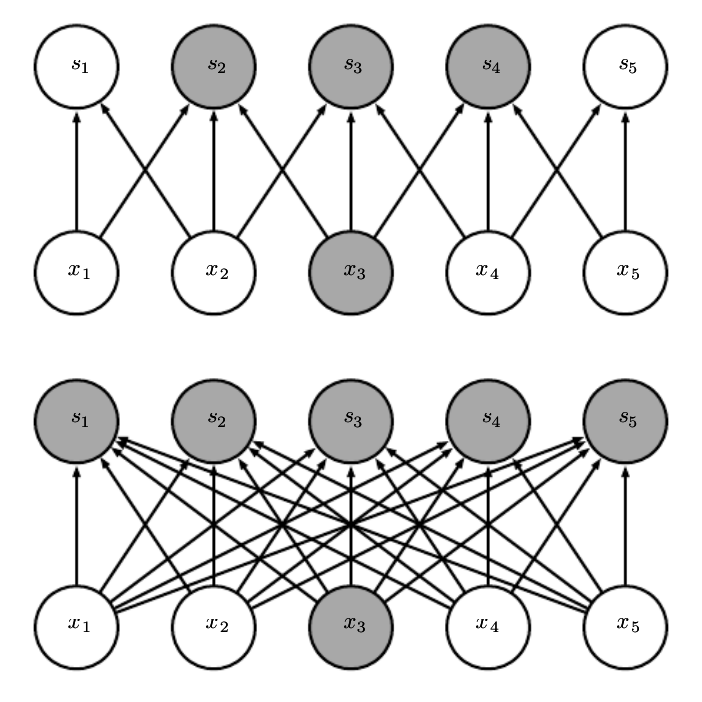
\includegraphics[width=0.5\linewidth]{media/sparce_connect_1.png}
	\caption{Sparse connectivity viewed from below. One input and the affected output units are highlighted in case of convolution with a kernel of size $3$ (top) and in case of dense layers with matrix multiplication (bottom). The figure is taken from \protect\hyperlink{Deeplea_Goodfellow}{Goodfellow et al (2016)}. }
	\label{sparse_connect_conv}
	\end{center}
\end{figure}

	\item \textbf{Equivariant representations:} as a consequence of the parameter sharing the convolutional layers have a property called equivariance to translations. A function $f(x)$ is equivariant to another function $g$, if $f\left(g(x)\right) = g\left(f(x)\right)$ (see figure \ref{commutative_diag_1}), so if the input changes, the output should change the same way. In case of convolution, if $g$ is any function that translates the input, then the convolution function is equivariant to $g$. To sum up, if we move the object in the input, its representation will move the same amount in the output.


\begin{figure}[h]
	\begin{center}
	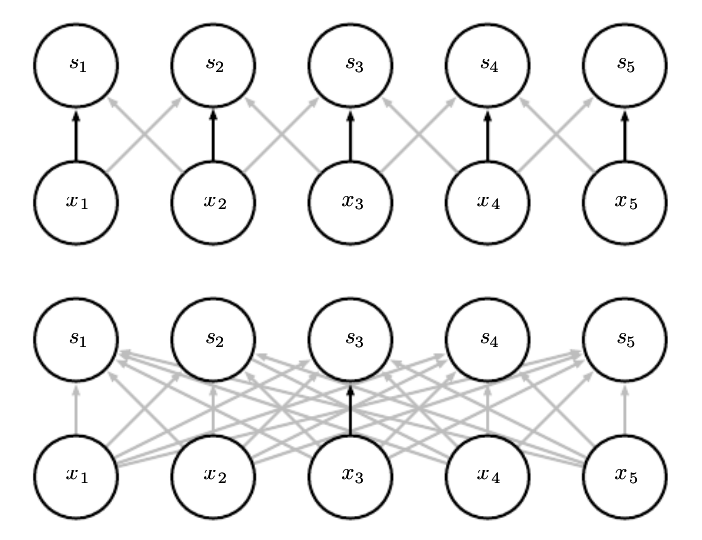
\includegraphics[width=0.5\linewidth]{media/parameter_sharing_conv.png}
	\caption{Parameter sharing in case of convolution with a kernel of size $3$ (top) and in case of a fully connected model (bottom). The figure is taken from \protect\hyperlink{Deeplea_Goodfellow}{Goodfellow et al (2016)}. }
	\label{parameter_sharing_conv}
	\end{center}
\end{figure}

\begin{figure}[h!]
	\begin{center}
	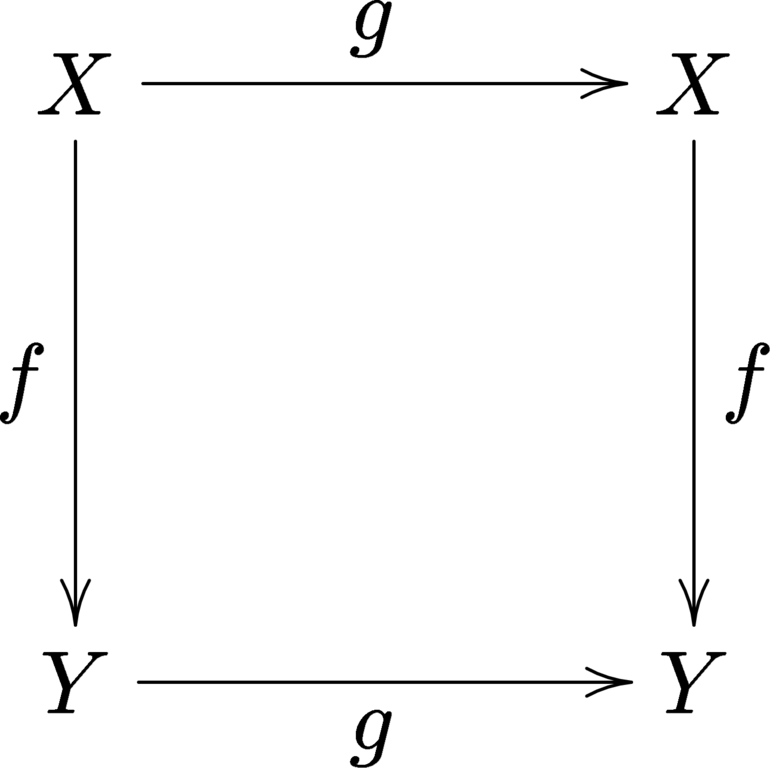
\includegraphics[width=0.3\linewidth]{media/Equivariant_commutative_diagram.png}
	\caption{Visualization of the equivariance property with the commutative diagram of $f$ and $g$. }
	\label{commutative_diag_1}
	\end{center}
\end{figure}
\end{itemize}

Notice that convolution is not naturally equivariant to other transformations, such as the rotation of the input image, but it can be achieved with the application of group theory.

\subsection{TODO}
batch normalization

autoencoders

word2vec

\newpage

\begin{thebibliography}{Nature}
%\bibliography{references}

\bibitem{Deeplea_Goodfellow}\hypertarget{Deeplea_Goodfellow}{}
Ian Goodfellow and Yoshua Bengio and Aaron Courville (2016). \textit{Deep learning}. MIT Press. \url{http://www.deeplearningbook.org}

\bibitem{Deeplea_LeCun_1}\hypertarget{Deeplea_LeCun_1}{}
LeCun, Y. (1989). Generalization and network design strategies. Technical Report, CRG-TR-89-4, University of Toronto. \url{http://yann.lecun.com/exdb/publis/pdf/lecun-89.pdf}

\bibitem{Deeplea_Rosenblatt_2}\hypertarget{Deeplea_Rosenblatt_2}{}
Rosenblatt, F. (1962). \textit{Principles of Neurodynamics}. Spartan, New York.

\bibitem{Deeplea_Rosenblatt_1}\hypertarget{Deeplea_Rosenblatt_1}{}
Rosenblatt, F. (1958). The perceptron: A probabilistic model for information storage and organization in the brain. \textit{Psychological Review}, \textbf{65}, 386–408.
\end{thebibliography}



\end{document}
